\documentclass[11pt]{article}
\usepackage{hyperref}
\usepackage{amsthm}
\usepackage{amsmath}
\usepackage{amsfonts}
\usepackage{tikz}
\usepackage{ wasysym }

\newtheorem{example}{Example}


\author{}
\title{}

\begin{document}
\pagenumbering{roman}
%\maketitle
{\Large
%Change Document name to: Graded Homework 1\_Jacob\_Nicholas
\noindent NAME:  Nicholas Jacob\\ 
EMAIL: \href{mailto: nicholascjacobphd@gmail.com}{nicholas.c.jacob-1@ou.edu}\\
STUDENT ID: \# 113578513\\
Final Project\\
COURSE: CS/DSA 4513 DATABASE MANAGEMENT\\ 
SECTION: ONLINE\\SEMESTER: FALL 2023\\
INSTRUCTOR:  DR. LE GRUENWALD\\
 SCORE:}

\newpage
\tableofcontents
\newpage
\pagenumbering{arabic}
\setcounter{page}{1}

\section{ER Diagram}
Here is my ER diagram

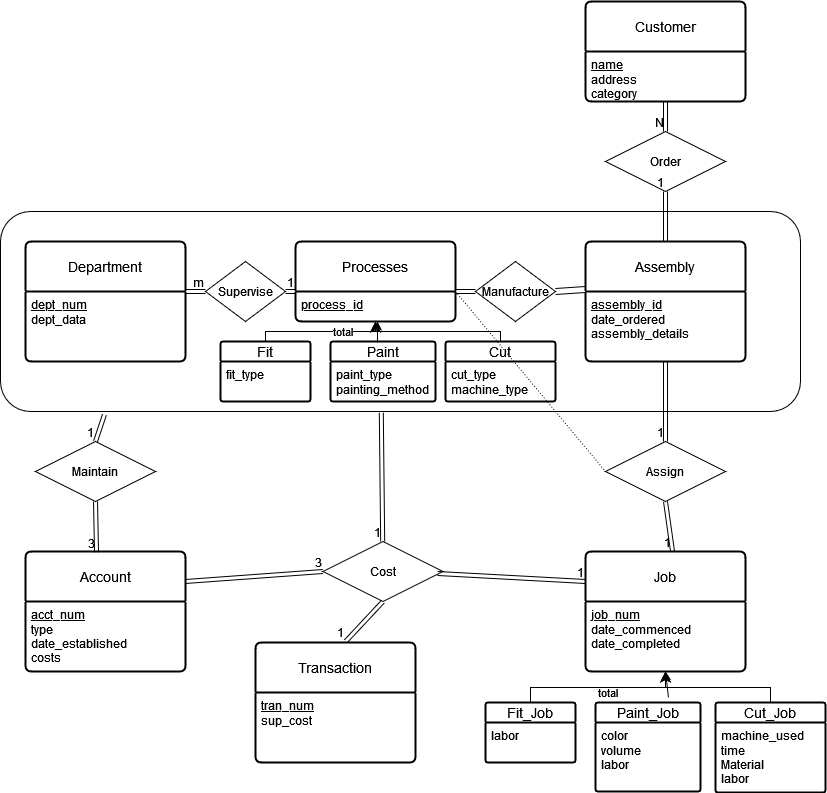
\includegraphics[width=\textwidth]{Project.png}
\newpage

\section{Relational Database Schema}

\indent Here are my schema:

Process(\underline{process\_id},process\_data)

Assemblies(\underline{ass\_id},ass\_details)

Create(\underline{process\_id},\underline{ass\_id})

Customer(\underline{name},address, category)

Orders(\underline{name},\underline{ass\_id})

Department(\underline{dept\_num},dept\_data)

Supervises(\underline{dept\_num},\underline{process\_id})

Fit(\underline{process\_id}, fit\_type)

Paint(\underline{process\_id}, paint\_type, painting\_method)

Cut(\underline{process\_id},cutting\_type, machine\_type)

Account(\underline{type}, \underline{acct\_id})

Job(\underline{process\_id}, \underline{ass\_id}, \underline{job\_num})

Account(\underline{type}, \underline{acct\_id})

Costs(\underline{job\_num},\underline{type}, \underline{acct\_id},\underline{process\_id}, \underline{ass\_id})

Fit\_Job(\underline{process\_id}, \underline{ass\_id}, \underline{job\_num}, labor)

Paint\_Job(\underline{process\_id}, \underline{ass\_id}, \underline{job\_num},color,volume, labor)

Cut\_Job(\underline{process\_id}, \underline{ass\_id}, \underline{job\_num}, machine\_type, time, material, labor)

\newpage
\section{Storage}

\begin{tabular}{|c|p{.75in}|c|p{.75in}|p{.75in}|p{.75in}|}\hline
Table Name & Query Number and Type & Search Key& Query Frequency& Selected File Organization & Justification\\ \hline\hline
Customer & 1 Insertion & name & 30/Day & Heap on name & At the moment adding lots of data is easiest with a heap.  I reserve the right to change this if we need to look for customers often...\\ \hline 
Department & 2 Insertion& dept\_num & infrequent & Sequential on dept\_num & Since this data is added infrequently but referenced by other tables often, sequential insertion seems appropriate.\\ \hline




\end{tabular}

\end{document}